\documentclass[12pt,a4paper]{article}
\usepackage{physics}
\usepackage{amssymb}
\usepackage{subcaption}
\usepackage{colortbl}
\usepackage{musicography}
\newcommand{\activity}{Activity 11 -- Basic video processing}
\input{spp.dat}

\begin{document}

\title{\TitleFont \activity}
\author[ ]{\textbf{Kenneth V. Domingo} \\
2015--03116 \\
App Physics 186, 1\textsuperscript{st} Semester, A.Y. 2019--20}
\affil[ ]{\corremail{kvdomingo@up.edu.ph} }

\maketitle
\thispagestyle{titlestyle}

\section*{Results and Discussion}
\setcounter{section}{1}

\subsection{Experimental phase}
For this activity \cite{soriano}, I paired up with Rene Principe and we decided to perform a simple experiment to obtain the acceleration due to gravity. We used a Nikon D3400 with a SIGMA 24-70mm lens. We set it to \texttt{ISO} 200, f/2.8, recording at 1080p60 at 50mm to eliminate any vignetting or lens distortion. We placed the camera on a tripod at a fixed distance away from a uniformly-lit wall and dropped a bright pink ball from rest such that its centroid was roughly aligned with the upper edge of the frame, and was allowed to freely fall. The bottom edge of the frame was aligned with the corner of the wall. The room was closed and there was no airconditioning, so we can assume that there are no significant forces pushing it away from its plane of fall. Using a caliper, the ball was determined to have a diameter of 6.5 cm.

\subsection{Computational phase}
\subsubsection{Preprocessing}
The raw video files were first trimmed in Adobe Premiere Pro such that the clip starts at the moment the ball is dropped and ends either when the ball stops bouncing or goes out of the frame. The video was then rotated into portrait mode such that the ground direction is downwards. Finally, it was exported as \texttt{mp4}. The original, unsegmented video can be accessed through \\
\url{https://drive.google.com/open?id=16IaBhmNCL8T7cAKvIIQ6y4vyOT1K08hK}.

\subsubsection{Segmentation and morphological cleaning}
Using Python, I first read an arbitrary frame such that the entire ball can be seen in the frame. Using my code for a previous activity on non-parametric segmentation, I selected the ROI such that it encompassed a rectangular portion of the ball, taking care not to include the background. After obtaining the ROI and its histogram, non-parametric segmentation can automatically detect the ball for all succeeding frames. Next, I applied Otsu's method to binarize the frames, followed by an elliptical closing operator of size $11 \times 11$. I then used the \texttt{regionprops} function from the \texttt{skimage} library to obtain the segmented ball's properties per frame, in particular the centroid and diameter properties. The result of these operations is shown in Fig. \ref{fig:segment}.

\subsubsection{Calibration}
The diameter of the ball was averaged for the first 30 frames (just before it bounces for the first time), and using the actual diameter obtained earlier, its pixel-to-length calibration is as follows:

\begin{equation}\label{eq:calibration}
	\mathrm{meters = pixels \times \frac{diameter (meters)}{diameter (pixels)}}
\end{equation}

Thus, the position of the ball in real units at any time can be obtained, and its velocity and acceleration can be computed using central difference algorithm. Its motion curves are shown in Fig. \ref{fig:motion}.

\subsubsection{Obtaining $g$}
Calculating the acceleration due to gravity $g$ can be done in two ways. First, we can isolate the position curve up to the point when it first bounces (first 30 frames), and fit this curve to an equation of the form

\begin{equation}\label{eq:curve-fit}
	f(t; g, v_0, x_0) = gt^2 + v_0 t + x_0
\end{equation}

\noindent
via nonlinear least-squares fitting. Using this method, we obtain a value of $\boxed{g = -9.68$ m/s$^2}$, which deviates by 1.31\% from the theoretical. For reference, the theoretical value is $g = -9.81$ m/s$^2$.

Another way this can be done is by taking again the first 30 frames and averaging their acceleration values which we obtained earlier. This method yields $\boxed{g = -9.61$ m/s$^2}$, which deviates by 2.04\% from the theoretical.

\begin{figure}[htb]
	\centering
	\begin{subfigure}[h!]{0.3\textwidth}
		\centering
		
\includegraphics[width=\textwidth]{7296/0.png}
		\caption{frame 1}
	\end{subfigure}
	\begin{subfigure}[h!]{0.3\textwidth}
		\centering
		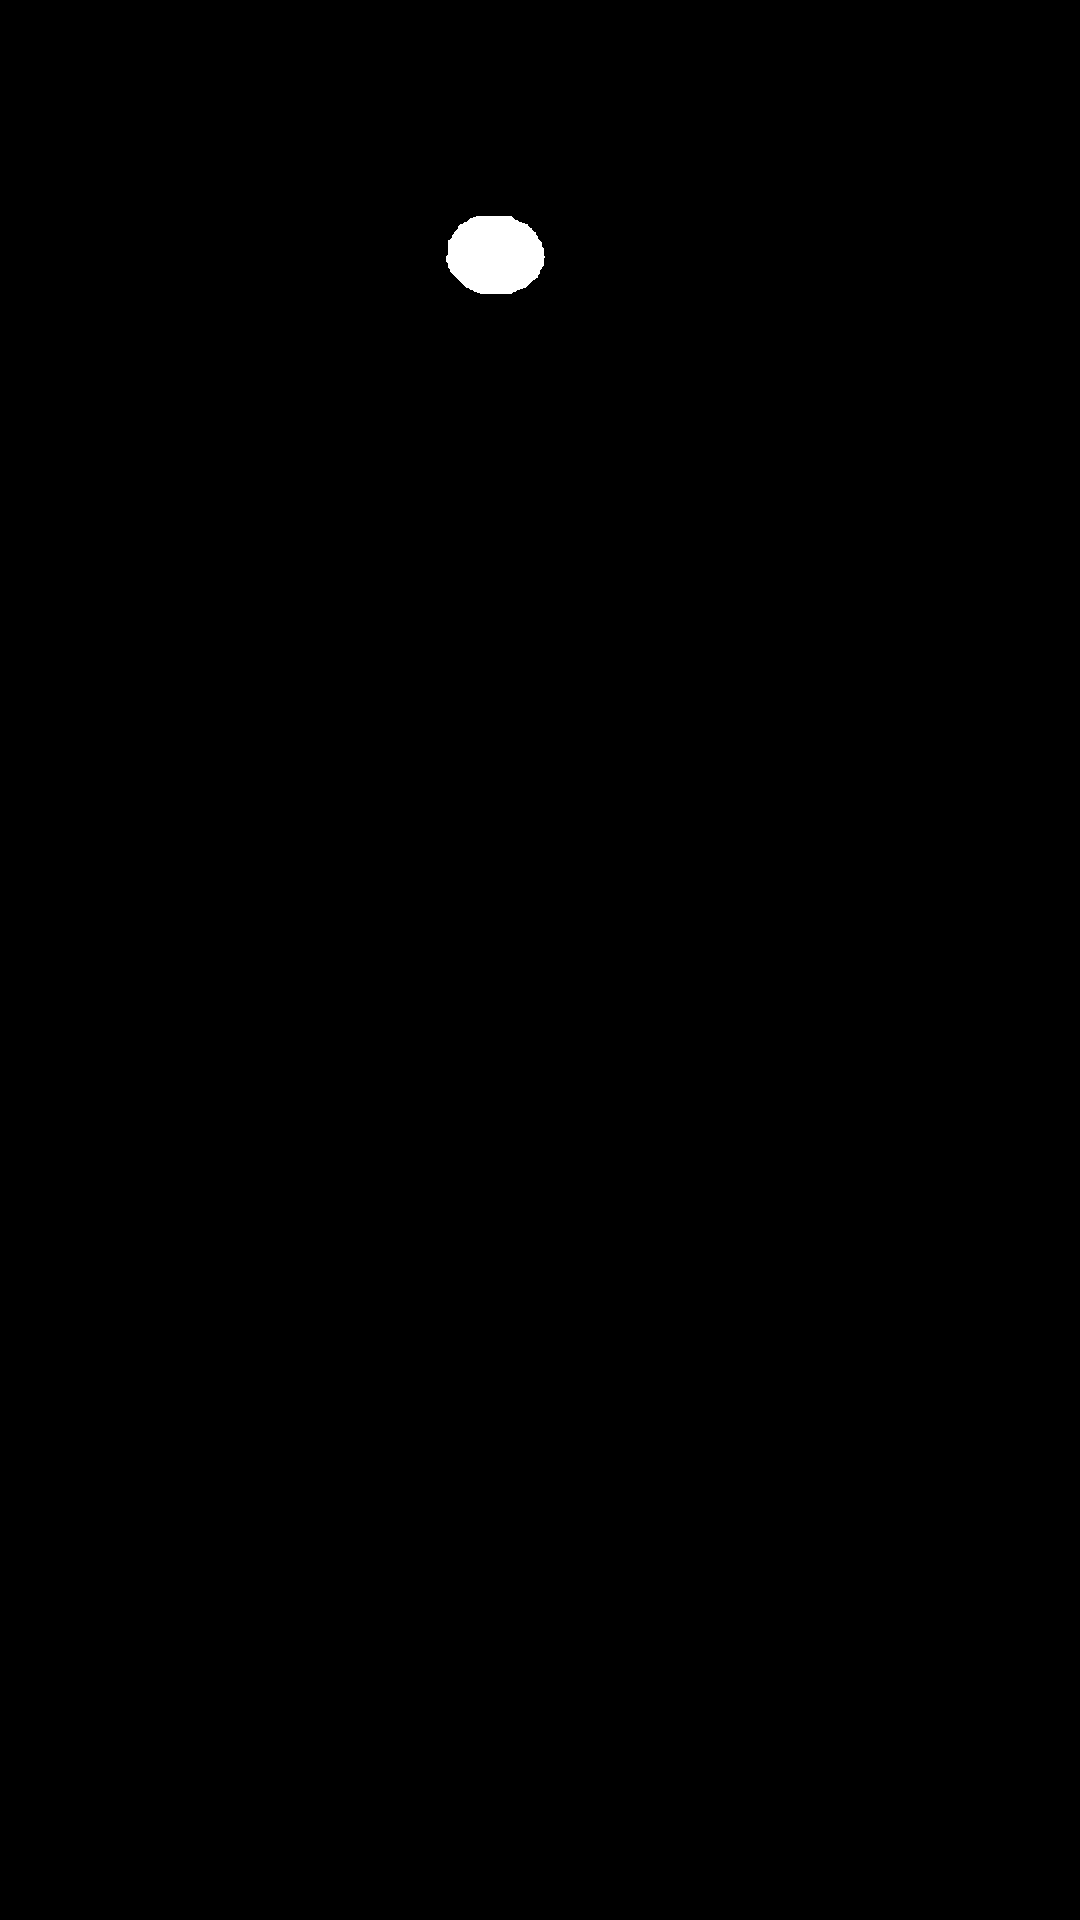
\includegraphics[width=\textwidth]{7296/9.png}
		\caption{frame 10}
	\end{subfigure}
	\begin{subfigure}[h!]{0.3\textwidth}
		\centering
		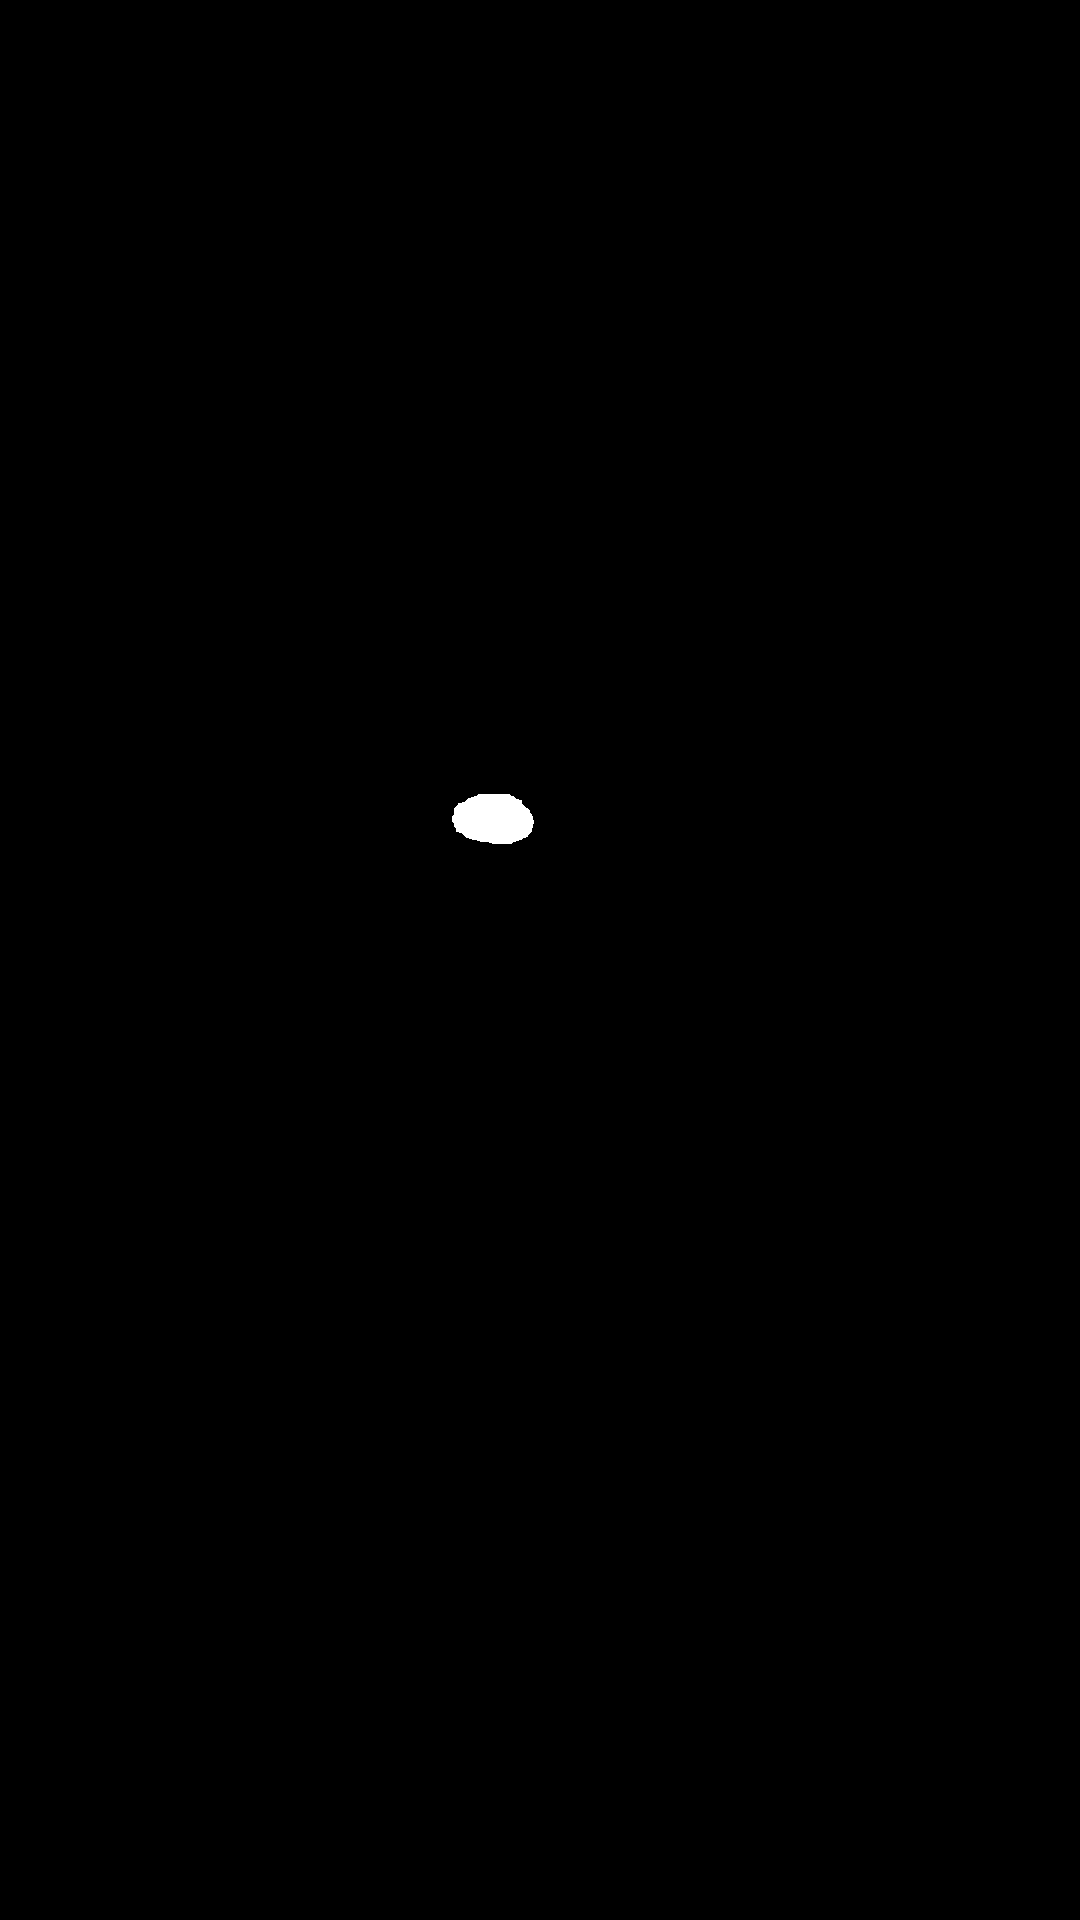
\includegraphics[width=\textwidth]{7296/18.png}
		\caption{frame 19}
	\end{subfigure}
	\begin{subfigure}[h!]{0.3\textwidth}
		\centering
		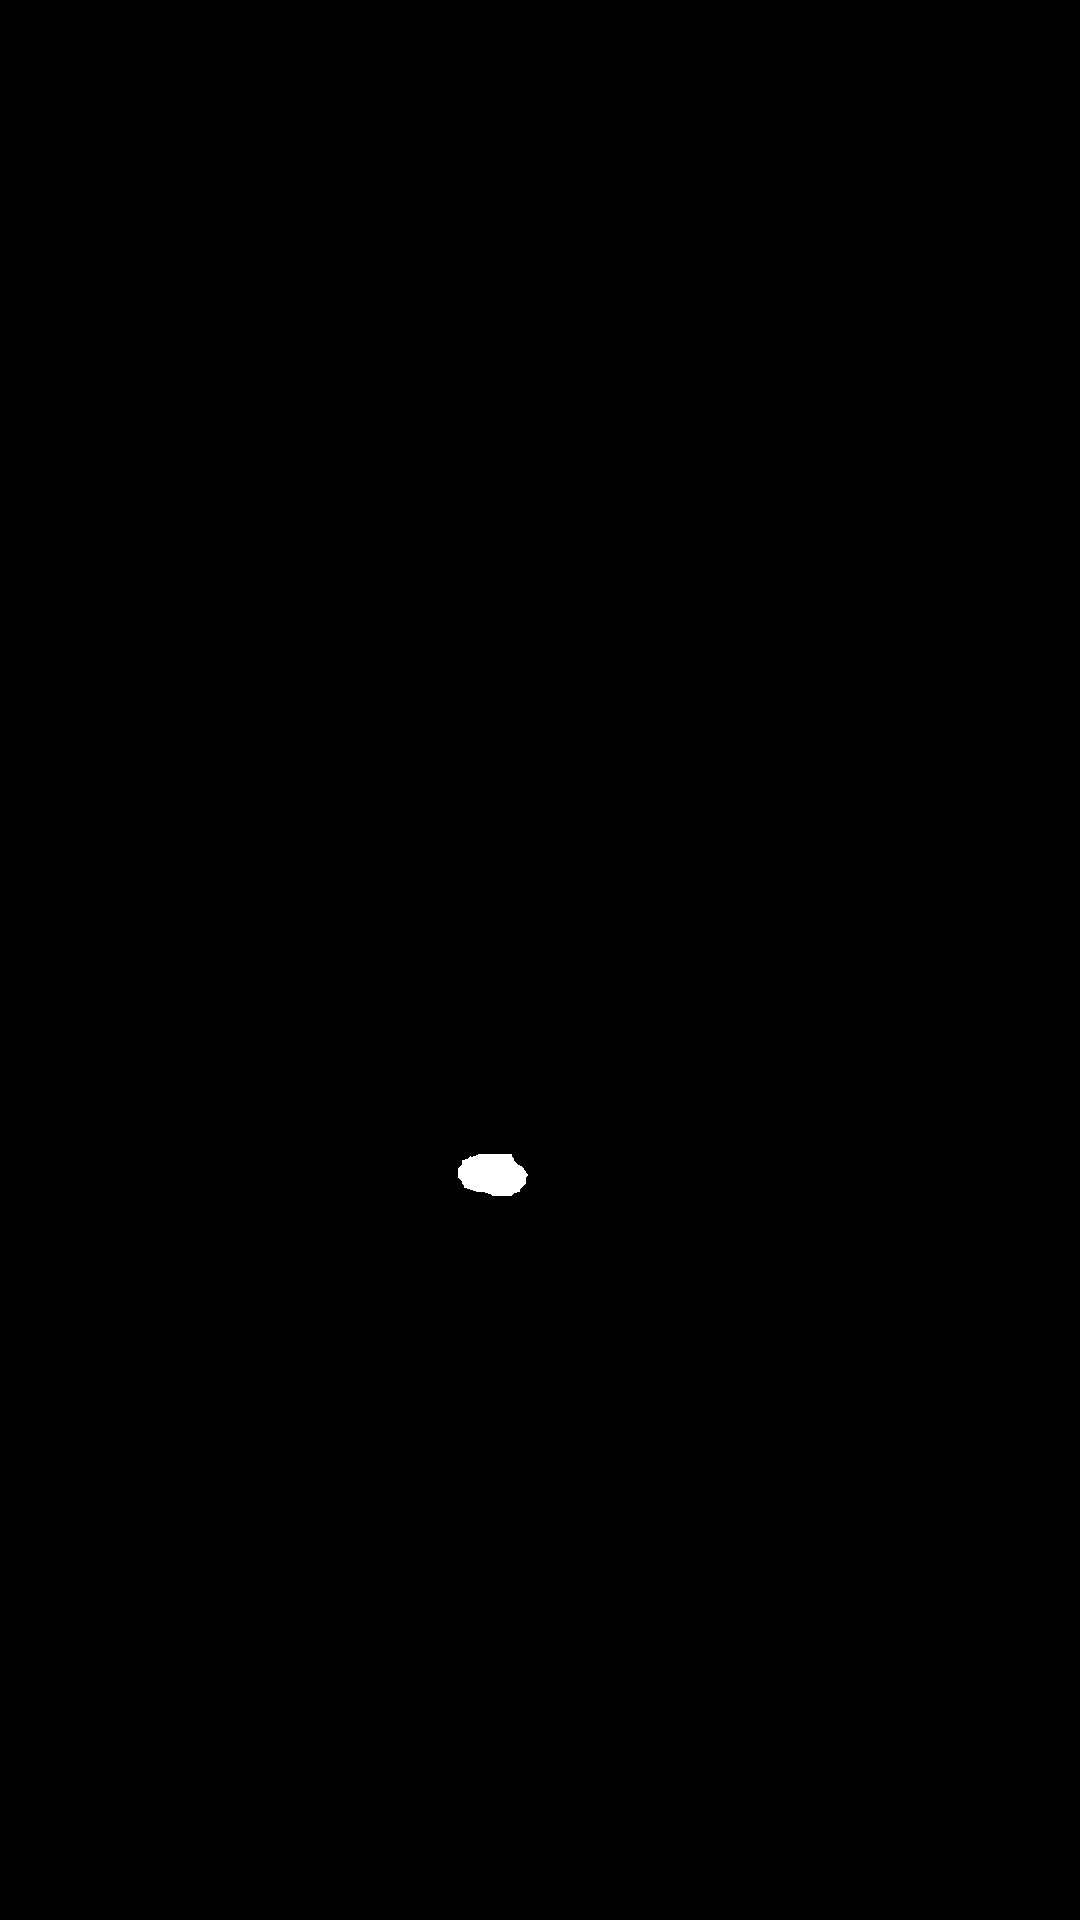
\includegraphics[width=\textwidth]{7296/22.png}
		\caption{frame 23}
	\end{subfigure}
	\begin{subfigure}[h!]{0.3\textwidth}
		\centering
		
\includegraphics[width=\textwidth]{7296/28.png}
		\caption{frame 29}
	\end{subfigure}
	\begin{subfigure}[h!]{0.3\textwidth}
		\centering
		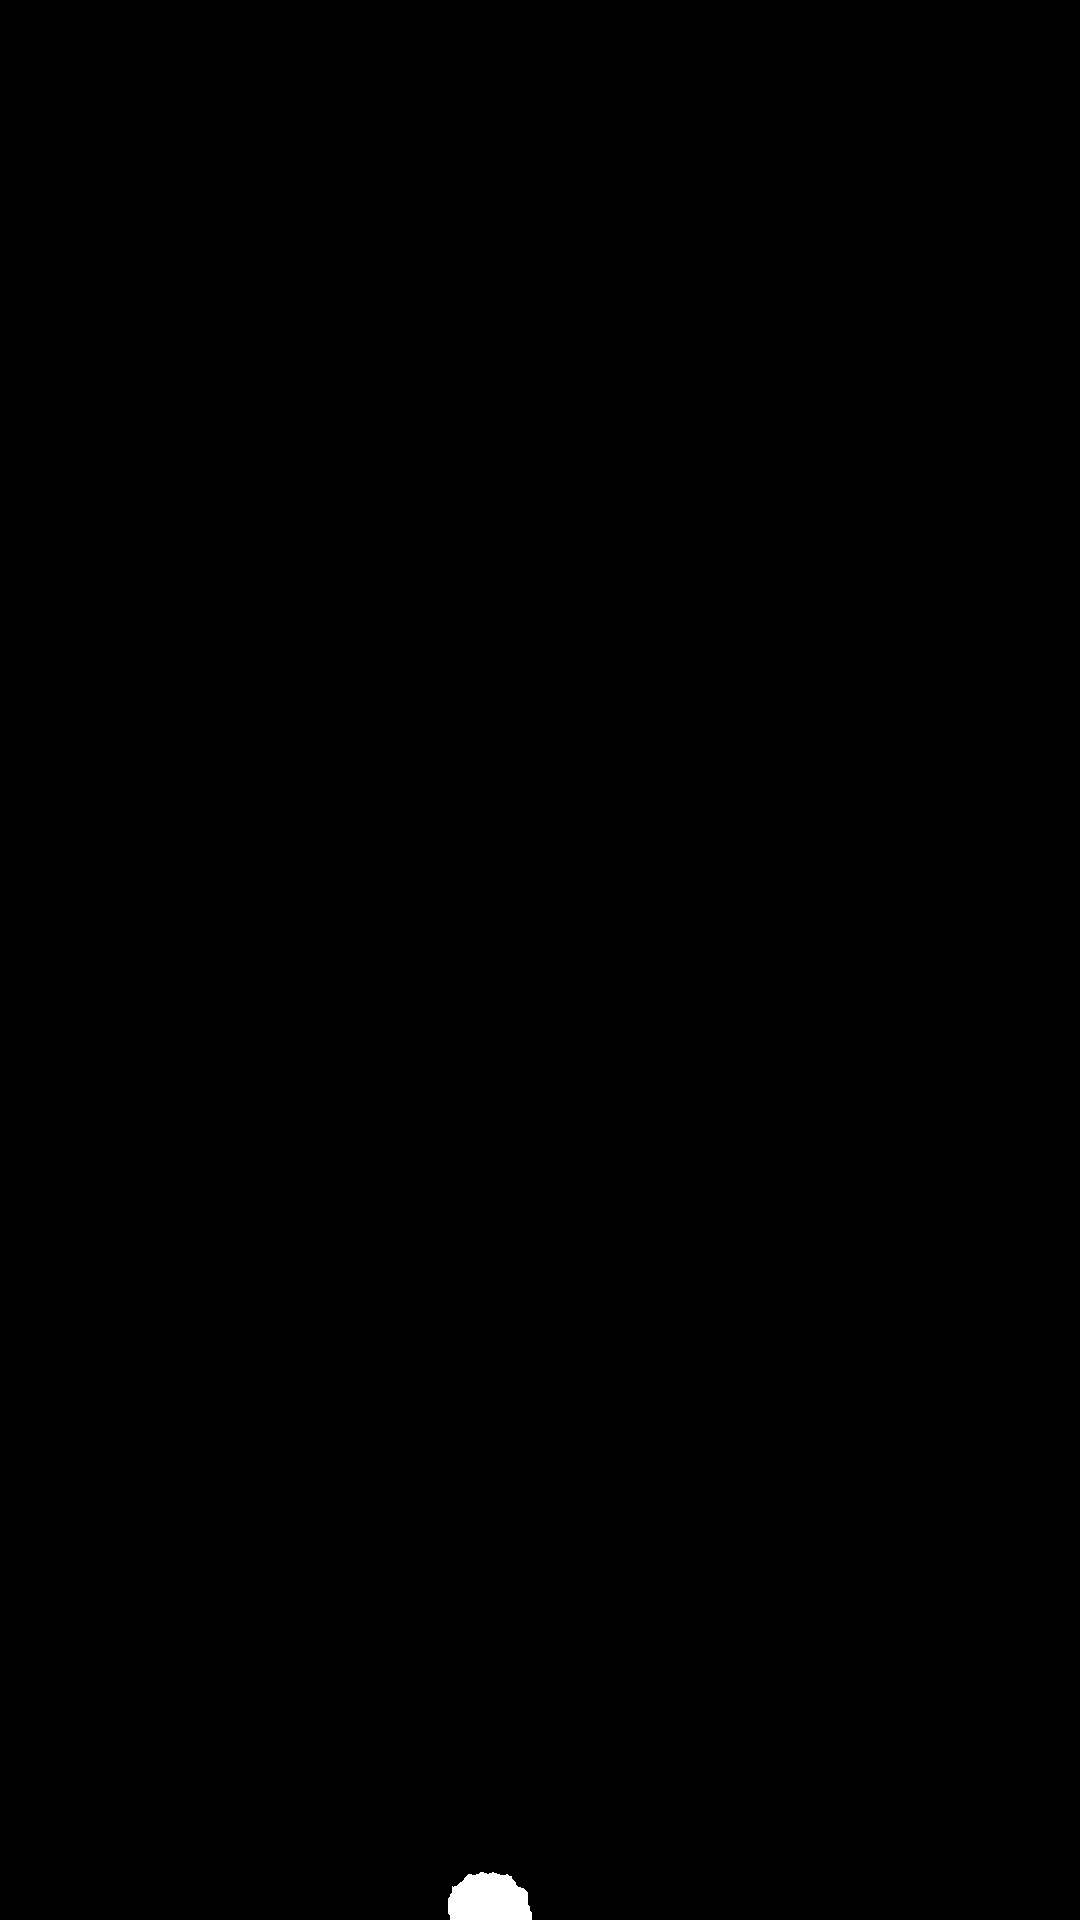
\includegraphics[width=\textwidth]{7296/29.png}
		\caption{frame 30}
	\end{subfigure}
	\caption{Representative frames as a result of successful segmentation and morphological cleaning. Notice in the middle frames that the ball appears to be squashed. This is due to the motion blur along the vertical, and in this case, the color of the ball starts to ``blend'' with the background. During this phenomenon, we measure the diameter horizontally, since there is no blur along this dimension.}
	\label{fig:segment}
\end{figure}

\begin{figure}[htb]
	\centering
	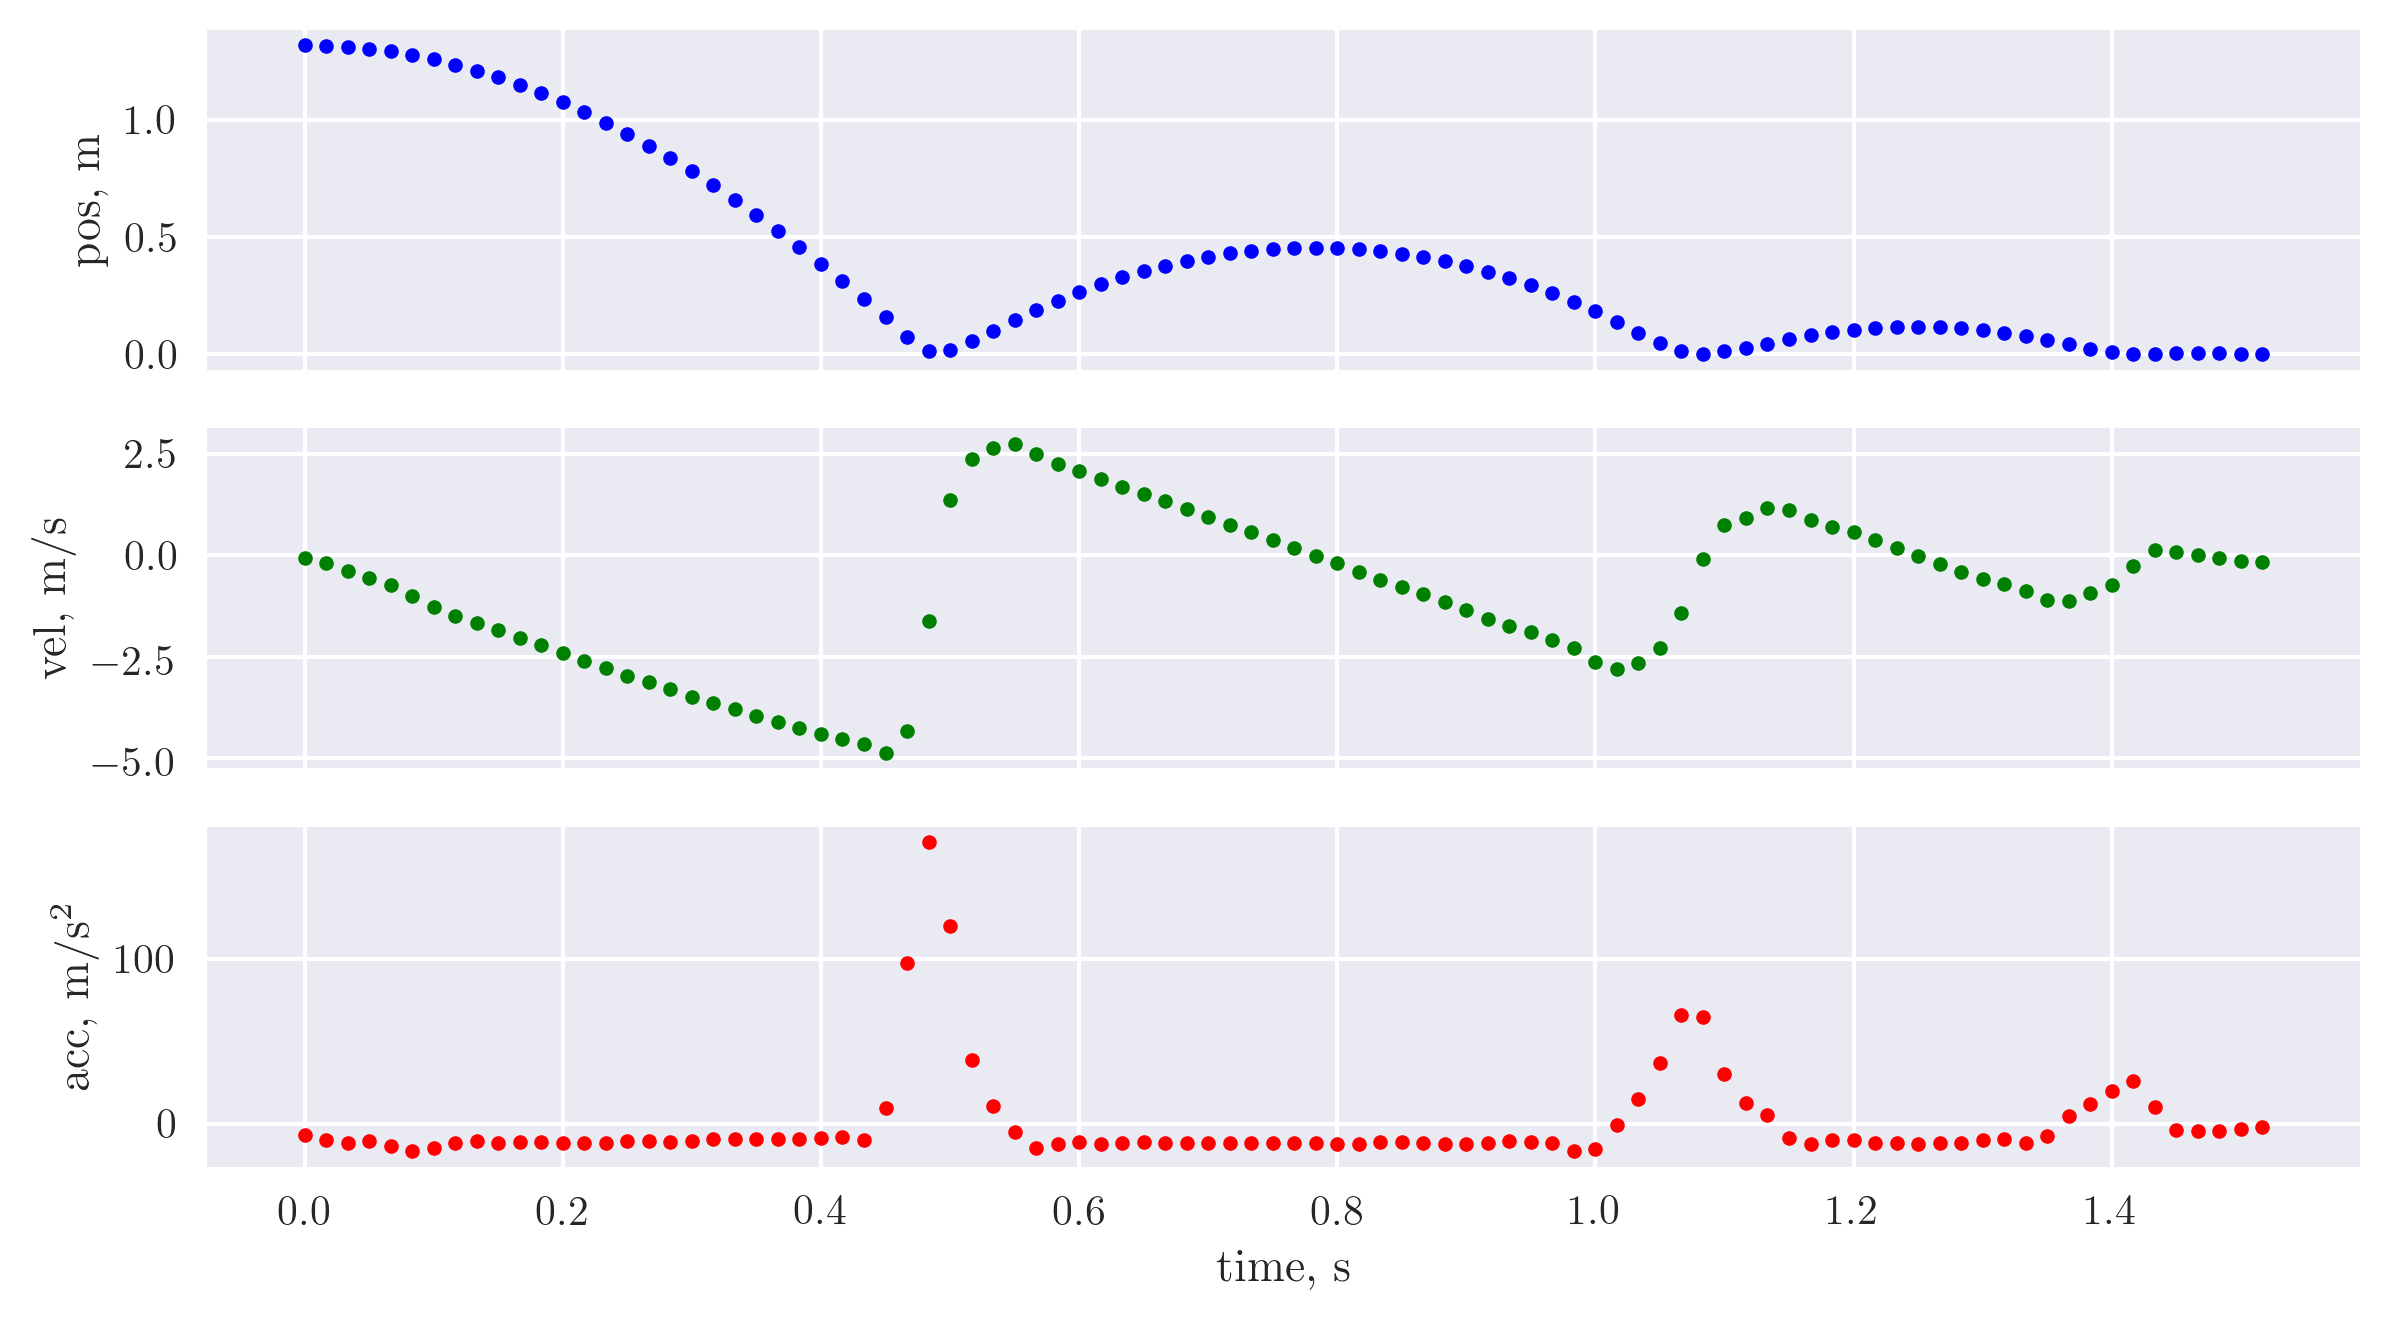
\includegraphics[width=\textwidth]{motion.png}
	\caption{Position, velocity \& acceleration curves of the free-falling ball.}
	\label{fig:motion}
\end{figure}

\clearpage
\begin{table}[!htb]
	\centering
	\caption{Self-evaluation.}
	\begin{tabular}{||r|c||}
		\hline
		Technical correctness & 5 \\ \hline
		Quality of presentation & 5 \\ \hline
		Initiative & 1 \\ \hline
		\textbf{TOTAL} & \textbf{11} \\ \hline
	\end{tabular}
	\label{tab:self-eval}
\end{table}

\bibliographystyle{spp-bst}
\bibliography{biblio}

\end{document}